\documentclass[11pt,oneside,a4paper]{report}

\begin{document}
\section{Types and validation}
The spell checking equivalent for computer programs could be type checking; a subproblem of validating a programmer's intuition of a program's intent.
Types also have other properties than simply validating they can in fact be related to theorems to which an implementation is the proof~\cite{howard1980formulae}.
\begin{lstlisting}[language=ML,caption={Head implementation},label={lst:headimpl},mathescape=true]
$\texttt{fun head l: List a} \rightarrow \texttt{a =}$
    $\texttt{match l}$
        $\texttt{| Cons x \_ } \rightarrow \texttt{x;}$
        $\texttt{| Nil} \rightarrow \texttt{?;}$
    ;
\end{lstlisting}
For instance, consider the implementation of the fuction with type $\texttt{List a} \rightarrow \texttt{a}$ in \autoref{lst:headimpl}.
A total implementation of the function cannot exist.

The type system for the $L$ language will be the Hindley-Milner type system~\cite{hindley1969principal,milner1978theory}.

\subsection{The language of types}
Before delving into types, the lambda calculus defined in \autoref{sec:lc} must be augmented with the \textit{let expression} (\autoref{eq:letb}).
\begin{align}
	\texttt{let } x = Y \texttt{ in } E
	\label{eq:letb}
\end{align}
It should be noted that the let binding can be expressed by abstraction and application (\autoref{eq:letaa}).
\begin{align}
	(\lambda x . E) (Y)
	\label{eq:letaa}
\end{align}
The let expression has a nice property that will become apparent later when typing rules are introduced.

Types are an artificial layer atop of a program just as spell checking is an artificial layer atop text.
There are two variants of types in the Hindley-Milner type system, the \textit{monotype} and the \textit{polytype}.
A monotype is either a type variable, an abstraction of two monotypes or an application of a type constructor (\autoref{eq:mono}).
\begin{align}
	mono \,\,\tau = a \,|\, \tau \rightarrow \tau \,|\, C \tau_1 \dots \tau_n
	\label{eq:mono}
\end{align}
\textit{Atoms} are terminal terms in a formula and are expressed either by type variable $a$ or $C$ with no type parameters.
The application term of the monotype is dependent on the primitive types of the programming language.
The types $\tau_1 \dots \tau_n$ are monotype parameters required to construct some type $C$.
In $L$ the set of type constructors are $\{ \texttt{Int}, \texttt{Bool} \} \cup \texttt{ADT}$.
\texttt{Int} and \texttt{Bool} are type constructors of arity 0 thus only have one instantiation and are atomic.
The set of constructors \texttt{ADT} encapsulates the set of program defined algebraic data structures (\autoref{adts}).
\begin{exmp}
    Let $\texttt{ADT} = \{ \texttt{List} \}$ where \texttt{List} is defined as in \autoref{lst:listadt}.
    The \textit{type constructor} (not to be confused for constructors like \texttt{Cons} or \texttt{Nil}) for \texttt{List} has the signature $\texttt{a} \rightarrow \texttt{List a}$ stating that if supplied with some type \texttt{a} it constructs a type of \texttt{List a} (effectively containing the provided type).
    The type \texttt{List} is a type constructor with one type parameter \texttt{a}.
\end{exmp}

$\bot$ denotes falsity, in type systems a value of this type can never exist since that in itself would disprove the program.
It is common in programming languages with strong type systems to let thrown exceptions be of type $\bot$ since it adheres to every type and indicates that the program is no longer running, since no instance of $\bot$ can exist.
$\top$ denotes truth, in type systems every type is a supertype of $\top$.
$\top$ is in practice only used to model side effects, since not all side effects return useful values.
In programming languages with side effects $\bot$ and $\top$ are considerably more useful than in pure programming languages.

A polytype is a polymorphic type (\autoref{eq:poly}).
\begin{align}
	poly \,\, \sigma = \tau \,|\, \forall a . \sigma
	\label{eq:poly}
\end{align}
Polymorphic types either take the shape of a type variable or introduce a type which all types $a$ adhere to. 
This does not necessarily include \textit{all} types since the \textbf{Gen} rule of \autoref{fig:hmrules} constrains the domain that $a$ ranges over to contain only bound type variables.
\begin{remark}
    All types adhere to a polymorphic type but polymorphic types do not adhere to any type other than polymorphic types.
    The concept of adherence in types is commonly called \textit{subtyping}.
    Every subtype is a \textit{at least} an implementation of it's supertype.
    Since this concept can be difficult to grasp from just text, observe \autoref{fig:polytree}.
    \begin{figure}[ht]
        \centering
            \begin{tikzpicture}
                \node[draw=none] (sigma) {$\sigma$};

                \node[draw=none, below = of sigma] (top) {$\top$};

                \node[draw=none, below = of top] (tv) {$\tau$};
                \node[draw=none, left = of tv] (arr) {$\tau_1 \rightarrow \tau_2$};
                \node[draw=none, right = of tv] (tc) {$C \tau_1 \dots \tau_n$};

                \node[draw=none, below = of tv] (bot) {$\bot$};

                \path [->] (sigma) edge node[left] {} (top);

                \path [->] (top) edge node[left] {} (arr);
                \path [->] (top) edge node[left] {} (tv);
                \path [->] (top) edge node[left] {} (tc);

                \path [->] (tv) edge node[left] {} (bot);
                \path [->] (arr) edge node[left] {} (bot);
                \path [->] (tc) edge node[left] {} (bot);
            \end{tikzpicture}
        \caption{The type hierarchy of Hindley-Milner.}
        \label{fig:polytree}
    \end{figure}
    Note that $\sigma$ is controversial to introduce to the type hierarchy and has only been so to illustrate the point of subtyping.
    $\sigma$ is but a mechanism to prove type systems, $\sigma$ is never a specific type.

\end{remark}
A principal component of typing in Hindley-Milner is the \textit{environment}.
The environment $\Gamma$ is a set of pairs of variable names and polytype (\autoref{eq:env}).
$\Gamma \vdash x: \sigma$ implies a \textit{typing judgment}, meaning that given $\Gamma$, the variable $x$ can adhere to the type $\sigma$.
\begin{remark}
    \label{remark:judgpoly}
    Judging a type does not necessarily mean that the judged type is the only type that $x$ may take, it states that it is one \textit{possible} type that $x$ may take.
    The property of taking multiple possible types is what allows polymorphism.
    This is made more apparent in \autoref{exmp:letpoly} where \texttt{id} may take the type of either $\forall a . a \rightarrow a$, $\texttt{Int} \rightarrow \texttt{Int}$ or $\forall a . (a \rightarrow a) \rightarrow (a \rightarrow a)$.
\end{remark}
\begin{align}
	\Gamma \,\, = \epsilon \,|\, \Gamma, x : \sigma
	\label{eq:env}
\end{align}

Like in the untyped lambda calculus, types also have notions of free and bound type variables.
Type variables are bound when they have been introduced by a quantification or exist in the environment.
\begin{align}
	 & \textit{free}(a) = \{ a \}                                                              \\
	 & \textit{free}(C \tau_1 \dots \tau_n ) = \bigcup_{i = 1}^n \textit{free}(\tau_i)           \\
     & \textit{free}(\tau_1 \rightarrow \tau_2) = \textit{free}(\tau_1) \cup \textit{free}(\tau_2)          \\
	 & \textit{free}(\Gamma) = \bigcup_{x:\sigma \in \Gamma} \textit{free}(\sigma)             \\
	 & \textit{free}(\forall a . \sigma) = \textit{free}(\sigma) - \{ a \}                     
	 %& \textit{free}(\Gamma \vdash x : \sigma) = \textit{free}(\sigma) - \textit{free}(\Gamma)
\end{align}
Free and bound type variables are a vital distinction for type analysis since \textbf{Gen} in \autoref{fig:hmrules} may only generalize over bound type variables.
The variables which may appear in a quantification have an important role in \autoref{eq:substitution}, since only free variables may be substituted.
\begin{exmp}
Consider the type for the function \texttt{fst} in \autoref{lst:fstimpl}.
\begin{lstlisting}[language=ML,caption={First function},label={lst:fstimplbad},mathescape=true]
fun fst a b: $\forall$A.$\forall$B.A $\rightarrow$ B $\rightarrow$ A = a;
\end{lstlisting}
\begin{lstlisting}[language=ML,caption={First function in lambda calculus},label={lst:fstimpl},mathescape=true]
let fst = $\lambda$a.(let f = $\lambda$b.a in f) in fst
\end{lstlisting}
    The type for \texttt{fst} is $\forall A \forall B . A \rightarrow B \rightarrow A$.

    Note that a naive typing could look like $\forall A  . A \rightarrow (\forall B . B \rightarrow A)$ but rank-2 polymorphism is not typable in Hindley-Milner.
    An important realization is the context from where the type analysis is made.
    If type analysis is made from within \texttt{f} the type of \texttt{f} becomes $\forall B . B \rightarrow A$ and the type variable $A$ is free.
\end{exmp}
\section{Hindley-Milner}
With the now introduced primitives, the Hindley-Milner type system is but a set of inference rules composed by said primitives.
\begin{figure}[ht]
	\begin{mdframed}
		\minipage{0.49\textwidth}
		\begin{prooftree}
			\AxiomC{$x: \sigma \in \Gamma$}
			\LeftLabel{Var}
			\UnaryInfC{$\Gamma\vdash x:\sigma$}
		\end{prooftree}
		\endminipage
		\minipage{0.49\textwidth}
		\begin{prooftree}
			\AxiomC{$\Gamma \vdash e_1 : \tau_1 \rightarrow \tau_2$}
			\LeftLabel{App}
			\AxiomC{$\Gamma \vdash e_2 : \tau_1$}
			\BinaryInfC{$\Gamma \vdash e_1 e_2 : \tau_2$}
		\end{prooftree}
		\endminipage\hfill\vspace{0.8cm}

		\minipage{0.49\textwidth}
		\begin{prooftree}
			\AxiomC{$\Gamma, x: \tau_1 \vdash e : \tau_2$}
			\LeftLabel{Abs}
			\UnaryInfC{$\Gamma \vdash \lambda x . e : \tau_1 \rightarrow \tau_2$}
		\end{prooftree}
		\endminipage\hfill
		\minipage{0.49\textwidth}
		\begin{prooftree}
			\AxiomC{$\Gamma \vdash e_1 : \sigma$}
			\LeftLabel{Let}
			\AxiomC{$\Gamma ,x : \sigma \vdash e_2 : \tau$}
			\BinaryInfC{$\Gamma \vdash \texttt{let } x = e_1 \texttt{ in } e_2 : \tau$}
		\end{prooftree}
		\endminipage\hfill\vspace{0.8cm}

		\minipage{0.49\textwidth}
		\begin{prooftree}
			\AxiomC{$\Gamma \vdash e : \sigma_1$}
			\AxiomC{$\sigma_1 \sqsubseteq \sigma_2$}
			\LeftLabel{Ins}
			\BinaryInfC{$\Gamma \vdash e : \sigma_2$}
		\end{prooftree}
		\endminipage\hfill
		\minipage{0.49\textwidth}
		\begin{prooftree}
			\AxiomC{$\Gamma \vdash e : \sigma$}
            \AxiomC{$a \notin \textit{free}(\Gamma)$}
			\LeftLabel{Gen}
			\BinaryInfC{$\Gamma \vdash e : \forall a . \sigma$}
		\end{prooftree}
		\endminipage
	\end{mdframed}
	\caption{Hindley-Milner type rules}
	\label{fig:hmrules}
\end{figure}
There are six rules in the Hindley-Milner rules outlined in \autoref{fig:hmrules}.
\begin{itemize}
    \item \textbf{Var} states that if some variable $x$ with type $\sigma$ exists in the environment, the type can be judged.
        In practice, when $x: \sigma$ is encountered in the expression tree it is added to the environment.
    \item \textbf{App} decides that if $e_1 : \tau_1 \rightarrow \tau_2$ and $e_2 : \tau_1$ has been judged to exist then $e_1 e_2$ implies the removal of $\tau_1$ from $\tau_1 \rightarrow \tau_2$ such that $e_1 e_2: \tau_2$.
    \item \textbf{Abs} is the typing rule of lambda abstractions.
        If $x : \tau_1$ exists in the environment from some type analysis of $e$ and the abstraction's body $e$ has been judged to be of type $\tau_2$ then the abstraction of $x$ must take the type of $x$ to create the type of the body $e$.
    \item \textbf{Let} states that if $e_1$ has been judged to have type $\sigma$ then the let expression's identifier $x: \sigma$ must exist in the environment when deriving the type of $e_2$.
        Observe that \textbf{Let} introduces a polymorphic type to the environment while \textbf{Abs} introduces a monomorphic one.
        Note that by \autoref{remark:judgpoly} $x$ may be polymorphic in $e_2$.
    \item \textbf{Inst} specializes some polymorphic type (in regard to the type system implementation) to a more specific polymorphic type.
        $\sqsubseteq$ is the partial order of types where the binary relation between two types compares the descriptiveness of types.
        \begin{exmp}
            In $L$ the smallest element is the top of the type hierarchy (\autoref{fig:polytree}), the polymorphic type.
        \end{exmp}
    \item \textbf{Gen} generalizes over all bound variables $a$.
\end{itemize}
Let polymorphism is exemplified in \autoref{exmp:letpoly}.

\begin{exmp}
\label{exmp:letpoly}
Throughout this example $(x, z)$ is the pair of the variables $x$ and $z$.

The identity function is a common example to illustrate type systems (\autoref{lst:idfun}).
\begin{lstlisting}[language=ML,caption={Identity function in $L$},label={lst:idfun}]
fun id x = x;
id 4;
\end{lstlisting}
\begin{lstlisting}[language=ML,caption={Identity function in lambda calculus with let},label={lst:idfunlam},mathescape=true]
let id = ($\lambda x . x$) in
id 4
\end{lstlisting}
Stating that id has the type $\forall a.a \rightarrow a$ and $4$ has the type \texttt{Int} is \autoref{lst:idfunlam} program correct?
By applying the Hindley-Milner rules one can prove or disprove this statement.
A correct proof of \autoref{lst:idfun} must be \autoref{fig:typeexampleid}.

\begin{lstlisting}[language=ML,caption={Identity function in lambda calculus by abstraction},label={lst:idfunlamabs},mathescape=true]
($\lambda$id.id 4)($\lambda$x.x)
\end{lstlisting}
\autoref{lst:idfunlam} and \autoref{lst:idfunlamabs} are two equivalent programs with slightly different proofs which raises the question of why the let expression is even needed.
If \autoref{lst:idfunlam} and \autoref{lst:idfunlamabs} were to be slightly changed such that two new programs \autoref{lst:idfunlam2} and \autoref{lst:idfunlamabs2} were to be proved, \autoref{lst:idfunlamabs2} would not be provable while \autoref{lst:idfunlam2} would.
\begin{lstlisting}[language=ML,caption={Identity function with two applications},label={lst:idfunlam2},mathescape=true]
let id = ($\lambda$x.x) in
(id 4, id id)
\end{lstlisting}
\begin{lstlisting}[language=ML,caption={Identity function with two applications as abstraction},label={lst:idfunlamabs2},mathescape=true]
($\lambda$id.(id 4, id id)($\lambda$x.x)
\end{lstlisting}
In \autoref{lst:idfunlamabs2} \texttt{id} cannot adhere to polymorphism by \textbf{Abs} in \autoref{fig:hmrules} whilst \textbf{Let} can.
%\begin{figure}[ht]
    %\begin{mdframed}[style=bigbox]
        %\begin{subfigure}[b]{1\textwidth}
        %\begin{prooftree}
                            %\AxiomC{$x : a \in \Gamma$}
                            %\LeftLabel{Var}
                        %\UnaryInfC{$\Gamma \vdash x : a$}
                    %\LeftLabel{Abs}
                %\UnaryInfC{$\Gamma \vdash (\lambda x . x) : a \rightarrow a$}
                    %\LeftLabel{Gen}
                    %\AxiomC{$a \notin \textit{free}(\Gamma)$}
                %\BinaryInfC{$\Gamma \vdash (\lambda x . x) : \forall a . a \rightarrow a$}
                %\AxiomC{$\forall a . a \rightarrow a \sqsubseteq \texttt{Int} \rightarrow \texttt{Int}$}
            %\LeftLabel{Inst}
            %\BinaryInfC{$\Gamma \vdash (\lambda x . x) : \texttt{Int} \rightarrow \texttt{Int}$}
        %\end{prooftree}
        %\caption{}
        %\label{fig:typewrongexampleid:1}
        %\end{subfigure}
        %\begin{subfigure}[b]{0.49\textwidth}
        %\begin{prooftree}
                    %\AxiomC{$\text{id} : \texttt{Int} \rightarrow \texttt{Int} \in \Gamma$}
                    %\LeftLabel{Var}
                %\UnaryInfC{$\Gamma \vdash \text{id} : \texttt{Int} \rightarrow \texttt{Int}$}
                    %\AxiomC{$4 : \texttt{Int} \in \Gamma$}
                    %\RightLabel{Var}
                %\UnaryInfC{$\Gamma \vdash 4 : \texttt{Int}$}
            %\RightLabel{App}
            %\BinaryInfC{$\Gamma, \text{ id} : \texttt{Int} \rightarrow \texttt{Int} \vdash $ id 4 : \texttt{Int}}
        %\end{prooftree}
        %\caption{}
        %\label{fig:typewrongexampleid:2}
        %\end{subfigure}
        %\begin{subfigure}[b]{0.49\textwidth}
        %\begin{prooftree}
                %\AxiomC{\ref{fig:typewrongexampleid:1}}
                %\AxiomC{\ref{fig:typewrongexampleid:2}}
            %\LeftLabel{Let}
            %\BinaryInfC{$\Gamma \vdash $ \texttt{let} id = $(\lambda x . x)$ \texttt{in} id 4: \texttt{Int}}
        %\end{prooftree}
        %\caption{}
        %\label{fig:typewrongexampleid:3}
        %\end{subfigure}
    %\end{mdframed}
    %\caption{Incorrect identity function instantiation proof}
    %\label{fig:typewrongexampleid}
%\end{figure}
\begin{figure}[ht]
    \begin{mdframed}[style=bigbox]
        \begin{subfigure}[b]{1\textwidth}
        \begin{prooftree}
                            \AxiomC{$\text{id} : \forall a . a \rightarrow a \in \Gamma$}
                            \LeftLabel{Var}
                        \UnaryInfC{$\Gamma \vdash \text{id} : \forall a . a \rightarrow a$}
                        \AxiomC{$\forall a . a \rightarrow a \sqsubseteq \texttt{Int} \rightarrow \texttt{Int}$}
                    \LeftLabel{Inst}
                    \BinaryInfC{$\Gamma \vdash \text{id} : \texttt{Int} \rightarrow \texttt{Int}$}
                        \AxiomC{$4 : \texttt{Int} \in \Gamma$}
                        \RightLabel{Var}
                    \UnaryInfC{$\Gamma \vdash 4 : \texttt{Int}$}
                \RightLabel{App}
                \BinaryInfC{$\Gamma, \text{ id} : \forall a . a \rightarrow a \vdash $ id 4 : \texttt{Int}}
        \end{prooftree}
        \caption{}
        \label{fig:typeexampleid:2}
        \end{subfigure}
        \begin{subfigure}[b]{0.49\textwidth}
        \begin{prooftree}
                                \AxiomC{$x : a \in \Gamma$}
                                \LeftLabel{Var}
                            \UnaryInfC{$\Gamma \vdash x : a$}
                        \LeftLabel{Abs}
                    \UnaryInfC{$\Gamma \vdash (\lambda x . x) : a \rightarrow a$}
                        \LeftLabel{Gen}
                        \AxiomC{$a \notin \textit{free}(\Gamma)$}
                    \BinaryInfC{$\Gamma \vdash (\lambda x . x) : \forall a . a \rightarrow a$}
        \end{prooftree}
        \caption{}
        \label{fig:typeexampleid:1}
        \end{subfigure}
        \begin{subfigure}[b]{0.49\textwidth}
        \begin{prooftree}
                \AxiomC{\ref{fig:typeexampleid:1}}
                \AxiomC{\ref{fig:typeexampleid:2}}
            \LeftLabel{Let}
            \BinaryInfC{$\Gamma \vdash $ \texttt{let} id = $(\lambda x . x)$ \texttt{in} id 4: \texttt{Int}}
        \end{prooftree}
        \caption{}
        \label{fig:typeexampleid:3}
        \end{subfigure}
    \end{mdframed}
    \caption{Identity function instantiation proof}
    \label{fig:typeexampleid}
\end{figure}
\end{exmp}



\subsection{Damas-Milner Algorithm W}
Typing rules are by themselves not that useful since they need all type information declared ahead of checking, inference attempts to guess types such that the rules are satisfied.
Type inference is the technique of automatically deriving types, of which there exist many algorithms.
One of the most common inference algorithms that produce typings which the Hindley-Milner rules accept is the Damas-Milner Algorithm W inference algorithm~\cite{damas1984type,damas1982principal}.

The Damas-Milner Algorithm W rules (\autoref{fig:dmrules}) introduce some new concepts such as \textit{fresh variables}, \textit{most general unifier}, and the \textit{substitution set}.
Fresh variables are introduced by picking a variable that has not been picked before from the infinite set $\tau_1, \tau_2 \dots $.
Fresh variables are introduced when unknown types are discovered and later unified.
The substitution set is a mapping from type variables to types (\autoref{eq:substitution}).
\begin{align}
    S = \{ a_1 \mapsto \tau_1, a_2 \mapsto \tau_2 \dots , a_n \mapsto \tau_n \} 
    \label{eq:substitution}
\end{align}
A substitution written $S T$ where $T$ is an arbitrary component of Hindley-Milner like an environment in which all type variables are substituted (\autoref{fig:subsem}).
\begin{figure}
\begin{mdframed}
\begin{align}
    &S \Gamma = \{ (x, S \sigma) \,\,|\,\, \forall (x, \sigma) \in \Gamma \} \tag{Environment}\\
    &S \sigma  = 
        \begin{cases}
            S \tau & \text{if } \sigma \equiv \tau\\
            \{ a' \mapsto \tau_1 \,\,|\,\, (a', \tau_1) \in S \,\,|\,\, (a, *) \notin S \} \sigma' & \text{if } \sigma \equiv \forall a . \sigma'
        \end{cases}
    \tag{Poly}\\
    &S (\tau_1 \rightarrow \tau_2) = S\tau_1 \rightarrow S\tau_2 \tag{Arrow}\\
    &S a = 
        \begin{cases}
            \tau & \text{if } (a, \tau) \in S\\
            a & 
        \end{cases}
    \tag{Typevariable}\\
    &S C \tau_1 \dots \tau_n = C S\tau_1 \dots S\tau_n \tag{Constructor}
\end{align}
\end{mdframed}
    \caption{Substitution semantics}
    \label{fig:subsem}
\end{figure}
Substitution sets can also be combined $S_1 \cdot S_2$ with well defined-semantics.
The combination of substitution sets is a key component for the correctness of the Damas-Milner inference algorithm.
\begin{align}
    S_1 \cdot S_2 = \{ (a \mapsto S_1\tau) \,\,|\,\, (a \mapsto \tau) \in (S_2 \cup_. S_1) \}
    \label{eq:combination}
\end{align}
The $\cup_.$ operator is distinct in the type variable and is left-biased (\autoref{eq:cupdot}).
\begin{align}
    S_1 \cup_. S_2 = S_1 \cup \{ (a \mapsto \tau) \,\,|\,\, (a \mapsto \tau) \in S_2 \,\,|\,\, (a, *) \notin S_1 \}
    \label{eq:cupdot}
\end{align}
\begin{remark}
By the substitution set combination operator transitive and circular substitutions cannot occur since type variables in $S_1$ will inherit all the mappings from $S_2$ and substitute ones that exist in both.
The properties ensured by the combination semantics also induce the property of idempotence.
This property is enforced by the Damas-Milner Algorithm W inference rules.
\end{remark}
Unification is performed differently based on the context.
Unification is performed on monotypes, each of which can take one of three forms (\autoref{eq:mono}).
Note that the Var rules for most general unifier outlined in \autoref{fig:mgu} are commutative.
\begin{figure}
	\begin{mdframed}
		\minipage{1\textwidth}
		\begin{prooftree}
			\AxiomC{$S, \{ (\tau_1 \rightarrow \tau_2, \gamma_1 \rightarrow \gamma_2) \} \cup T $}
			\LeftLabel{Arrow}
			\UnaryInfC{$S,T \cup \{ (\tau_1, \gamma_1), (\tau_2, \gamma_2) \}$}
		\end{prooftree}
		\endminipage\hfill\vspace{0.8cm}

		\minipage{0.39\textwidth}
		\begin{prooftree}
            \AxiomC{$\tau_1, \tau_2$}
            \LeftLabel{Intro}
			\UnaryInfC{$\emptyset, \{ (\tau_1, \tau_2) \}$}
		\end{prooftree}
		\endminipage
		\minipage{0.59\textwidth}
		\begin{prooftree}
			\AxiomC{$S, \{ (a, \tau_1) \} \cup T$}
			\AxiomC{$a \equiv \tau_1$}
			\LeftLabel{
				Var empty
			}
			\BinaryInfC{$S, T $}
		\end{prooftree}
		\endminipage\hfill\vspace{0.8cm}

		\minipage{1\textwidth}
		\begin{prooftree}
			\AxiomC{$S, \{ (a, \tau_1) \} \cup T $}
			\AxiomC{$a \notin \textit{free}(\tau_1)$}
			\LeftLabel{Var sub}
			\BinaryInfC{$S \cup \{ a \mapsto S\tau_1 \}, \{ a \mapsto S\tau_1 \} \cup T$}
		\end{prooftree}
		\endminipage\hfill\vspace{0.8cm}

		\minipage{1\textwidth}
		\begin{prooftree}
			\AxiomC{$S,C_1 \tau_1 \dots \tau_n,C_2 \gamma_1 \dots \gamma_n \cup T$}
			\AxiomC{$C_1 \equiv C_2$}
			\LeftLabel{Atom}
			\BinaryInfC{$S , \{ (\tau_1, \gamma_1) \dots , (\tau_n, \gamma_n)\} \cup T$}
		\end{prooftree}
		\endminipage\hfill\vspace{0.8cm}
	\end{mdframed}
	\caption{Rules for most general unification}
	\label{fig:mgu}
\end{figure}

%\begin{lemma}
	%Var sub and Var empty are commutative.
%\end{lemma}
%\begin{proof}
	%Var empty is trivially true since $\equiv$ is commutative and for any $a$ and $\tau_1$ the rule produces $\emptyset \cup T = T$.\\\\
    %The commutative property of Var sub comes from the realization that $S \cup \{ \tau_1 \mapsto S\tau_2 \}$ and $S \cup \{ \tau_2 \mapsto S\tau_1 \}$ lets Algorithm W accept on the same inputs.
    %Furthermor note that Algorithm W substitutes and combines substitution sets at every step of the expression tree such that transitive types never occur because of the combination semantics.
    %\begin{case}
        %The types $\tau_1$ and $\tau_2$ are first introduced and used in unification.
        %Either all future uses of $\tau_1$ will be mapped to $\tau_2$ by the substitution set or all future uses of $\tau_2$ will be mapped to $\tau_1$.
    %\end{case}
    %\begin{case}
        %$\tau_1$ has been assigned in an earlier unification.
        %If $\tau_2 \mapsto \tau_1$ any existing references to $\tau_1$ need not change since all expressions of type variable $\tau_2$ will be mapped by the rules defined in \autoref{fig:hmrules}.
        %If any future rules need the type variable $\tau_1$ and $\tau_1 \mapsto \tau_2$ is introduced to the substitution set, the substitution rules in \autoref{fig:hmrules} will substitute the type.
    %\end{case}
%\end{proof}
An important implementation detail which should be noted is that of the polymorphic type.
Polymorphic types can be regarded as being a pair of bound types and monotype.
This representation is convenient for the \textbf{Gen} rule.

Moreover an additional adjustment must be made before allowing the implementation of an inference algorithm.
The \textbf{Inst} rule has slightly different semantics.
\begin{remark}
    The Damas-Milner algorithm W is the most popular inference algorithm for Hindley-Milner.
    Though it remains the most popular, it has some interesting competitors.
    One of which is that of the constraint solver approach which is also used in OCaml~\cite{heeren2002generalizing}.
    The constraint solver approach is a two phase type inference algorithm.
    In the first phase the algorithm inspects the expression tree and generates a set of constraints as it goes.
    After the set of constraints $C$ has been generated it then traverses the constraints and generates type variable substitutions.
    It is argued that error reporting is significantly easier in such an approach.
\end{remark}
\begin{figure}
	\begin{mdframed}[style=style1]
		\minipage{0.40\textwidth}
		\begin{prooftree}
			\AxiomC{$x: \sigma \in \Gamma$}
			\AxiomC{$\tau = \textit{inst}(\sigma)$}
			\LeftLabel{Var}
			\BinaryInfC{$\Gamma \vdash x:\tau , \emptyset$}
		\end{prooftree}
		\endminipage\hfill
		\minipage{0.64\textwidth}
		\begin{prooftree}
			\AxiomC{$\tau_1 = \textit{fresh}$}
			\AxiomC{$\Gamma, x: \tau_1 \vdash e: \tau_2, S$}
			\LeftLabel{Abs}
			\BinaryInfC{$\Gamma \vdash \lambda x . e : S\tau_1 \rightarrow \tau_2, S$}
		\end{prooftree}
		\endminipage\hfill\vspace{0.8cm}

		\minipage{1\textwidth}
		\begin{center}
			App
		\end{center}
		\vspace{-0.7cm}
		\begin{prooftree}
			\AxiomC{$\Gamma \vdash e_1 : \tau_1, S_1 \,\,\,\, \tau_3 = \textit{fresh}$}
			\AxiomC{$S_1 \Gamma \vdash e_2 : \tau_2, S_2 \,\,\,\, S_2 = \textit{mgu}(S_2 \tau_1, \tau_2 \rightarrow \tau_3)$}
			\BinaryInfC{$\Gamma \vdash e_1 e_2 : S_2 \tau_3, S_3 \cdot S_2 \cdot S_1$}
		\end{prooftree}
		\endminipage\hfill\vspace{0.8cm}

		\minipage{1\textwidth}
		\begin{prooftree}
			\AxiomC{$\Gamma \vdash e_1 : \tau_1, S_1$}
			\AxiomC{$S_1 \Gamma , x : S_1 \Gamma(\tau_1) \vdash e_2 : \tau_2, S_2$}
			\LeftLabel{Let}
			\BinaryInfC{$\Gamma \vdash \texttt{let } x = e_1 \texttt{ in } e_2 : \tau_2, S_1 \cdot S_2$}
		\end{prooftree}
		\endminipage
	\end{mdframed}
	\caption{Algorithm W}
	\label{fig:dmrules}
\end{figure}
Another interesting addition introduced by algorithm W in \autoref{fig:dmrules} is \textit{inst}.
\textit{inst} naturally follows from the \textbf{Inst} rule in \autoref{fig:hmrules} but has a slightly different behaviour.
The \textit{inst} function does not specify types anymore but simply makes unification possible.
\[
    \textit{inst}(\sigma) = \{ \, a \,\,|\,\, \forall a \,\,|\,\, a \notin \textit{free}(\sigma) \, \}
\]
\begin{remark}
In the language $L$ functions \texttt{fun} translate to let expressions while \texttt{let} translates to abstraction and application.
\end{remark}
\subsection{Recursion}
Recursion is a trivial matter once the primitives of the Hindley-Milner type system have been introduced.
Recall that in \autoref{sec:lamrec} recursion (along with mutual recursion) was shown to be implementable by introducing functions to their own scope, the same is true for types.
Allowing recursive functions in Hindley-Milner type inference systems is a matter of letting the function be present in the environment when inferring the function's own body.
\begin{exmp}
If the function \texttt{f} defined in \autoref{lst:recplus1} were to be typed it would need to be introduced as an unknown type to the environment before typing the body of \texttt{f}.
\begin{lstlisting}[language=ML,caption={Recursive function},label={lst:recplus1},mathescape=true]
fun f x = (f x) + 1;
\end{lstlisting}
Let $\Gamma = \{ \texttt{f} : \forall \tau . \tau, \texttt{x} : \forall \mu . \mu \}$.
From the application \texttt{f x} the unification \texttt{unify}$(\tau, \gamma \rightarrow \mu) = \{ \tau \mapsto \mu \rightarrow \gamma \}$ must be performed, and the resulting type for the expression is $\gamma$.
The addition operation forces \texttt{unify}$(\texttt{Int}, \gamma) = \{ \gamma \mapsto \texttt{Int} \}$.
Finally the application of the addition function $+: \texttt{Int} \rightarrow \texttt{Int} \rightarrow \texttt{Int}$ and the two expressions \texttt{f x} and $1$ such that the resulting expression type is \texttt{Int}.

\end{exmp}

\section{The cost of expressiveness}
Modern languages with strong type systems tend to be notoriously slow to type on pathelogical inputs.
In fact many languages with strong type systems provide type systems expressive enough to be turing complete.

In the construction of the compiler for $L$ one target was the C++ language.
An instance of a pathological input for the C++ type checker is most definitely the untyped lambda calculus.
The lambda terms in C++ must adhere to polymorphism in many cases which has some unknown but large blowup in compilation time.
In fact type polymorphism is commonly the root of blowup in typing.

ML which implemented Hindley-Milner was believed to have linear complexity before shown to be exponential.
As it will turn out, Hindley-Milner also suffers an explosive worst case induced by a pathological input fueled by polymorphism.

\begin{lemma}
    Hindley-Milner typing is worst case $O(c^n)$.
\end{lemma}
\begin{proof}
    The basis of the blowup stems from the introduced fresh type variables in the polymorphic let inference rule.
    If the amount of type variables can be shown to be exponential the running time must be at least the same by operations such as subsection set combination and unification.
\begin{lstlisting}[language=ML,caption={Nested pair},label={lst:pairproof},mathescape=true]
fun dup a f = f a a;
fun deep x = dup (dup (dup ($\dots$ x)));
\end{lstlisting}
    \autoref{lst:pairproof} builds a large function signature for \texttt{deep}.
    The innermost \texttt{pair} invocation will have it's signature unified to $x \rightarrow (x \rightarrow x \rightarrow \tau) \rightarrow \tau$.
    The second innermost \texttt{pair} invocation has the signature $((x \rightarrow x \rightarrow \tau) \rightarrow \tau) \rightarrow (((x \rightarrow x \rightarrow \tau) \rightarrow \tau) \rightarrow \gamma) \rightarrow \gamma$.
    Naively one might judge \autoref{lst:pairproof} to run in $O(2^n)$ but an important observation for why \autoref{lst:pairproof} does not induce exponential blowup is the uniqueness of the type variables.
    If an efficient representation of \texttt{dup} was implemented such that the left and right side were shared such that $\mu \mapsto ((x \rightarrow x \rightarrow \tau) \rightarrow \tau)$, the amount introduced type variables would be $O(n)$.
\begin{lstlisting}[language=ML,caption={Nested pairs with different type variables},label={lst:pairproofexp},mathescape=true]
fun tuple a b f = f a b;
fun one = tuple tuple tuple;
fun two = tuple one one;
fun three = tuple two two;
$\dots$
\end{lstlisting}
    The trick to induce an exponential running time is with the pathological program in \autoref{lst:pairproofexp}.
    By allowing \texttt{tuple} to be polymorphic and have having $c > 1$ polymorphic parameters, every time \texttt{tuple} is instantiated it will contain only fresh variables.
    The type of \texttt{tuple} is $a \rightarrow b \rightarrow (a \rightarrow b \rightarrow c) \rightarrow c$.
    Clearly this looks very much like \autoref{lst:pairproof} but has the subtle difference of letting the parameters \texttt{a} and \texttt{b} be polymorphic and introducing every ''step`` as a polymorphic let expression.
    The return type of \texttt{one} (the type of \texttt{f}) is displayed in \autoref{eq:instexp}.
    \begin{align}
        \textit{inst}(a \rightarrow b \rightarrow (a \rightarrow b \rightarrow c) \rightarrow c) \rightarrow \textit{inst}(a \rightarrow b \rightarrow (a \rightarrow b \rightarrow c) \rightarrow c) \rightarrow \gamma \rightarrow \gamma.
        \label{eq:instexp}
    \end{align}
    The first and second instantiations will contain different type variable such that they are not structurally equivalent \autoref{eq:afterinstexp}.
    \begin{align}
        (\tau \rightarrow \mu \rightarrow (\tau \rightarrow \mu \rightarrow \phi) \rightarrow \phi) \rightarrow (\varphi \rightarrow \zeta \rightarrow (\varphi \rightarrow \zeta \rightarrow \delta) \rightarrow \delta) \rightarrow \gamma \rightarrow \gamma.
        \label{eq:afterinstexp}
    \end{align}
\end{proof}
Running the program \autoref{lst:pairproofexp} in $L$ yields a blowup of $2^n$ (\autoref{lst:appedix:bigexp}).
\autoref{fig:expplot} shows the relationship between the program in $L$, the theoretical time and an exp fit of data from $L$.
\begin{figure}[ht]
    \centering
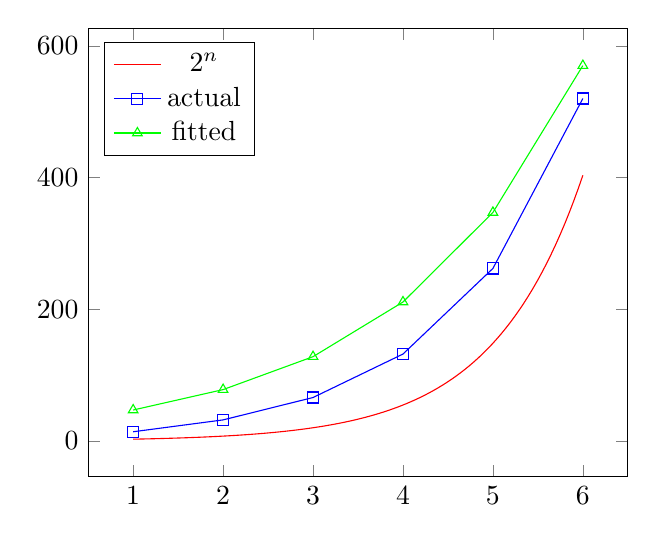
\begin{tikzpicture}
    \begin{axis}[
        legend pos= north west
        ]
       \addplot[
            domain=1:6,
            samples=100,
            color=red
        ]{exp(x)};
        \addlegendentry{$2^n$}

        \addplot[
            color=blue,
            mark=square
        ]
        coordinates {
(1,14)  (2,32)  (3,66) (4,132) (5,262) (6,520)
        };
        \addlegendentry{actual}

        \addplot[
            color=green,
            mark=triangle
        ]
        coordinates {
(1,47)  (2,78) (3,128) (4,211) (5,347) (6,570)
        };
        \addlegendentry{fitted}

   \end{axis} 
\end{tikzpicture}
    \caption{Plot of type variables in Hindley-Milner type systems}
    \label{fig:expplot}
\end{figure}

\end{document}
